\section{When the billiard is swept non-monotonically}
\label{sec:05-non-monotonic}

In \cref{prop:05-locus-x100}, we saw that $X_{100}$ sweeps the elliptic billiard in the direction opposite to the motion of billiard 3-periodic vertices.

The next triangle center on \cite{etc} which is on the $X_9$-centered circumconic is $X_{88}$, known to be collinear with $X_1$ and $X_{100}$. Assume a monotonic traversal of billiard 3-periodic vertices along the billiard. It turns out at a certain aspect ratio, the ``motion'' of $X_{88}$ can be made to stop. 

\begin{proposition}
At $a/b=\alpha_{88}$, the y velocity of $X_{88}$ vanishes when the 3-periodic is a sideways isosceles, where 
\[\alpha_{88}=(\sqrt{6+2\sqrt{2}}\,)/2\simeq{1.485} \]
\end{proposition}

\begin{proof}
Parametrize a 3-periodic vertex $P_1(t)=[a \cos{t},b \sin{t}]$. At $t=0$, $P_1=(a,0)$ it can be easily checked that $X_{88}=(-a,0)$. Solve $y_{88}'(t)|_{t=0}=0$ for $a/b$. After some algebraic manipulation, this equivalent to solving $4x^4-12x^2+7=0$, whose positive roots are $(\sqrt{6\pm 2\sqrt{2}}\,)/2$. $\alpha_{88} $ is the largest of the two.
\end{proof}

Indeed, there are three types of $X_{88}$ motion with respect to $P_1(t)$: (i) $a/b<\alpha_{88}$: monotonic and opposite to $P_1(t)$; (ii) $a/b=\alpha_{88}$: monotonic and opposite, but with full stop at the billiard major vertices; (iii) $a/b<\alpha_{88}$: non-monotonic, containing two retrograde phases.

An equivalent statement, illustrated in \cref{fig:05-x88-envelope}, is that the line family $X_1 X_{100}$ is instantaneously tangent to its {\em envelope} at $X_{88}$. Referring to Figure~\ref{fig:05-x88-envelope}:

\begin{proposition}
Over billiard 3-periodics, the envelope of $X_1 X_{100}$ is (i) entirely inside, (ii) touches at vertices of, or (iii) intersects the billiard, for $a/b$ (i) less than, (ii) equal to, or (iii) greater than $\alpha_{88}$, respectively. 
\label{prop:05-x88-env}
\end{proposition}

Interestingly:

\begin{proposition}
The motion of $X_{88}$ is instantaneously (i) opposite to $P_1$, (ii) stationary, or (iii) in the direction of $P_1$, if the tangency $E$ of $X_1 X_{100}$ with the envelope lies inside, on, or outside the billiard.
\label{prop:05-x88-envelope}
\end{proposition}

\begin{figure}
    \centering
    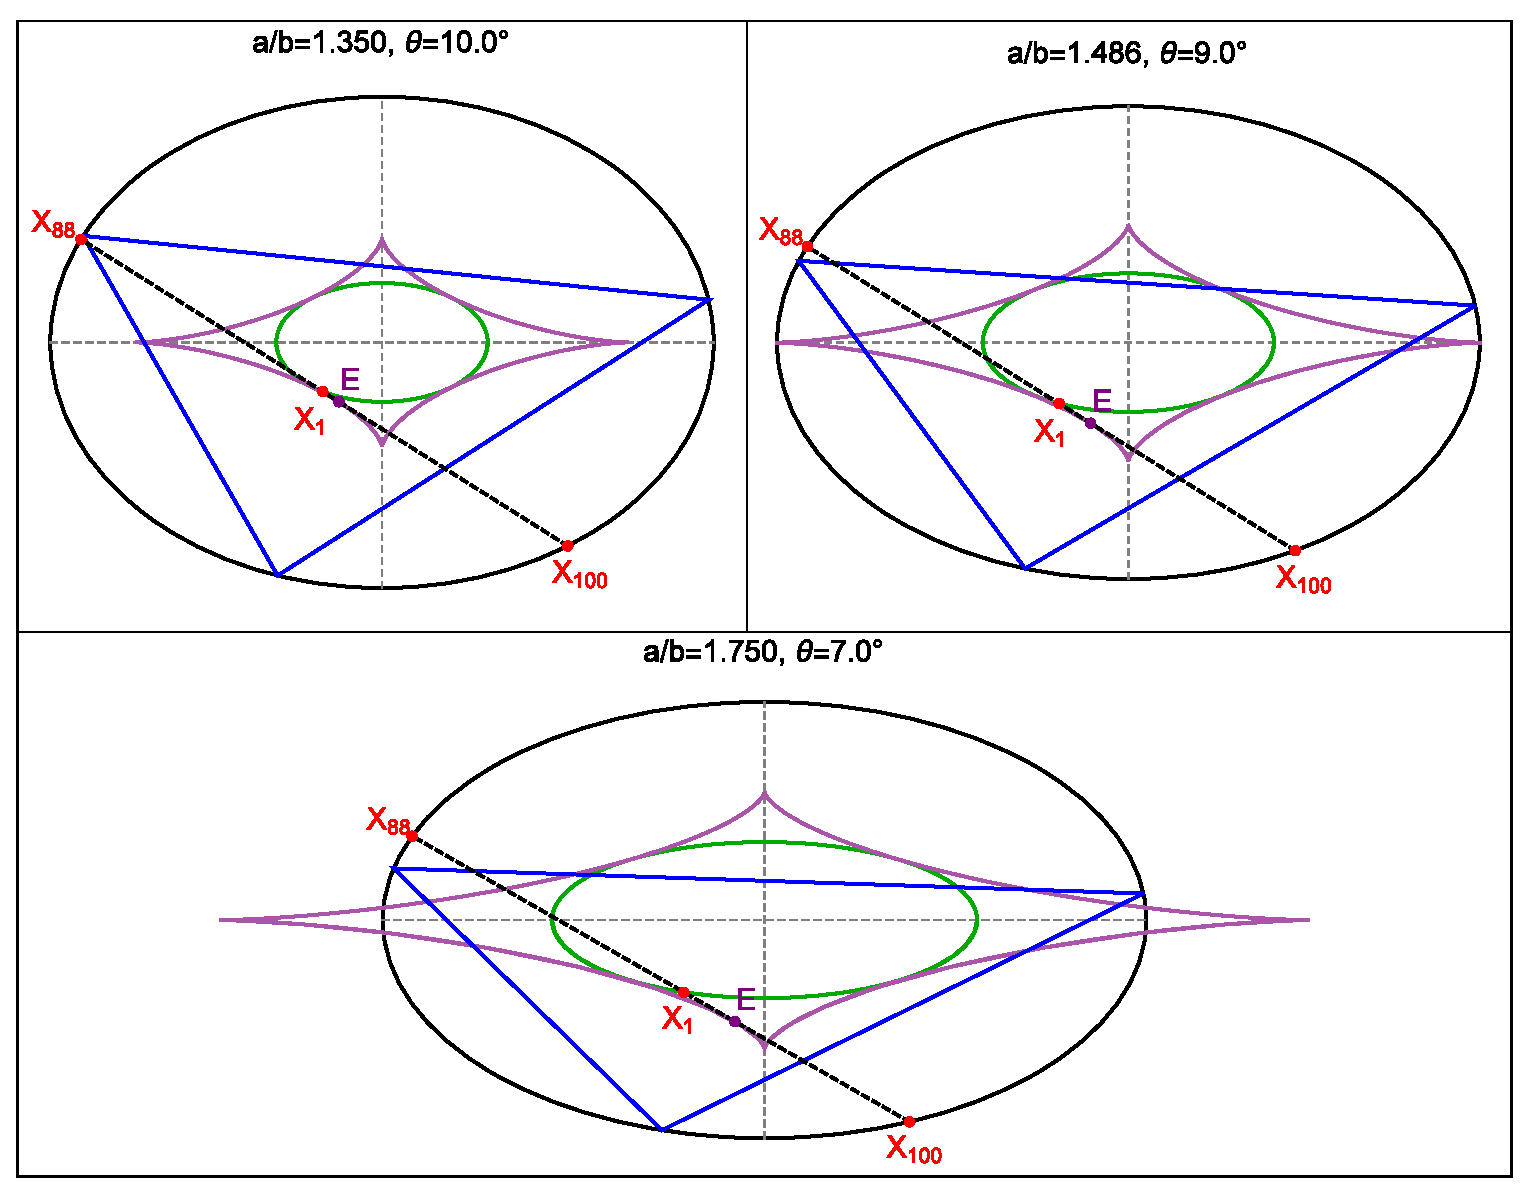
\includegraphics[width=\textwidth]{pics_05_190_trio}
     \caption{Collinear points $X_1,X_{100},X_{88}$ shown in an elliptic billiard with $a/b$ (i) less than (top-left), (ii) equal to (top-right), or (iii) greater than (bottom), $\alpha_{88}{\simeq}1.486$. The motion of $X_{88}$ relative to 3-periodic vertices will be: (i) monotonic and opposite to the vertices, (ii) monotonic and opposite but will full stops at the vertices, and (iii) non-monotonic. The envelope (purple) of line  $X_1 X_{100}$ intersects the billiard if $a/b>\alpha_{88}$ (bottom). The motion of $X_{88}$ is instantaneously (i) opposite to $P_1$, (ii) stationary, or (iii) in the direction of $P_1$, if the tangency $E$ of $X_1 X_{100}$ with the envelope lies inside, on, or outside the billiard. \href{https://youtu.be/nJLp--JjDZU}{Video}, \href{https://bit.ly/3hKicgM}{Live}}
    \label{fig:05-x88-envelope}
\end{figure}